\begin{frame} \frametitle{Supplementary Slides}
\end{frame}

\begin{frame} \frametitle{RK45 Formula}
	\centering
	\begin{figure}
		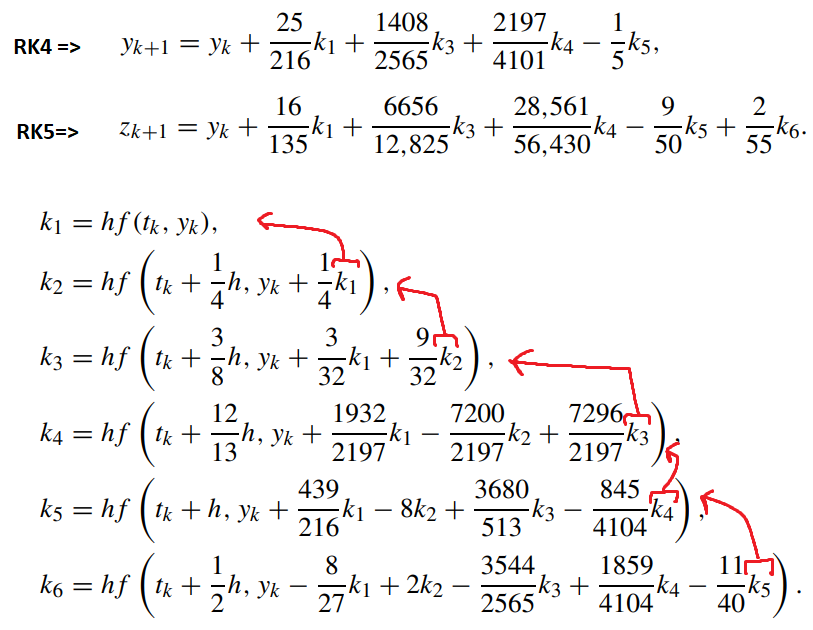
\includegraphics[width=0.8\textwidth]{./fig/rk45.png}
	\end{figure}
\end{frame}


\begin{frame}[c] \frametitle{ Syntax changes to allow smooth-token calculation }
	\begin{block}{Description}
		\begin{itemize}
			\item To allow calculation of smooth-token of higher than 1st order, we need more differential equation information.
		\end{itemize}
	\end{block}
	\begin{block}{Changes}
		\begin{itemize}
			\item The vector field $f$ definition is changed to indicate the differentiation order.
			\begin{itemize}
				\item $f : \mathbf{L} \times 2^X \times 2^I \times \mathbb{N}_{\geq 1} \rightarrow \mathbb{R}^n$.
				\item E.g., $f(l,\overrightarrow{x}, \overrightarrow{i}, 2) = x_i^{(2)}$.
			\end{itemize}
			\item The vector field $h$ definition is changed to indicate the differentiation order.
			\begin{itemize}
				\item $h : \mathbf{L} \times 2^X \times 2^I \times \mathbb{N}_{\geq 0} \rightarrow \mathbb{R}^n$.
				\item E.g., $h(l,\overrightarrow{x}, \overrightarrow{i}, 3) = o_i^{(3)}$.
			\end{itemize}
		\end{itemize}
	\end{block}
\end{frame}

\begin{frame}[c] \frametitle{ Smooth-token Calculation / Exchange }
	\begin{block}{Proposition}
		\begin{myitemize}
			\item The $(m+1)$th differential equations in QSHIOA are always depends on lower order values up to $m$.
			\item E.g., we have a coupled ODEs, $\dot{x} = xy$ and $\dot{y} = y - x$.
			\item $\ddot{x} = \frac{dx}{dt} y + x \frac{dy}{dt} = \dot{x}y + \dot{y}x$, $\quad \ddot{y} = \dot{y} - \dot{x}$.
			\item $\dddot{x} = \ddot{x}y + 2\dot{x}\dot{y} + \ddot{y}x$, $\quad \dddot{y} = \ddot{x} - \ddot{y}$.
		\end{myitemize}
	\end{block}
	\begin{block}{Calculation Dependency}
		\begin{itemize}
			\item From the proposition, the calculation of any $(m+1)$th order ODE depends on the values of $m$th order.
			\item So, there is a dependency.
		\end{itemize}
	\end{block}
\end{frame}

\begin{frame}[c] \frametitle{Overcoming the stationary point execution inefficiency}
	\begin{block}{Cause}
		\begin{itemize}
			\item The rate of change is almost zero due to the extremely small/zero gradient.
			\item Many iterations are needed to narrow down to the point where the approximations intersect with the $\Delta q$ threshold.
		\end{itemize}
	\end{block}
	\begin{block}{Proposing approach}
		\begin{itemize}
			\item When we reach the maximum iteration depth, and still could not reach narrow enough, we need to somehow force move the time.
			\item Current implementation has a configuration parameter called $escape_time$, which is a fixed value.
			\item Since we have the guards already in Taylor polynomials, we should be able to use the error estimation formula (remainder theorem -- Lagrange formula). 
			\item $R(t) = \frac{f^{(n+1)}(c)}{(n+1)!}t^{(n+1)}$
			\item Where, $c$ is a value between $(0, t)$. It is important that this is an open interval!
		\end{itemize}
	\end{block}
\end{frame}

\begin{frame}[c] \frametitle{Result Section}
	\begin{block}{What are we going to show?}
		\begin{itemize}
			\item We are going to show the comparison of three methods:
			\begin{enumerate}
				\item RK45: this will be used from Simulink/Stateflow.
				\item MQSS: Although the proof is not for multivariate functions, MQSS still can be executed.
				\item Proposed one.
			\end{enumerate}
		\end{itemize}
	\end{block}
\end{frame}

\begin{frame}[c] \frametitle{ Recap: Quantised State Hybrid Input Output Automata (QSHIOA) }
	\begin{block}{Definition}
		$\mathcal{H}_{q} = \langle L, X, X_q, V, O, Init, f, f_q, h, Inv, E,
		  G, R\rangle $
		\begin{itemize}
		\item $L = \{l_{0},\ldots,l_{n}\}$ a set of discrete locations.
		\item $V$ is a finite collection of input variables.
		\item $O$ is a finite collection of output variables.
		\item $X$ is a finite collection of continuous variables.
		\item $Init \subseteq \{l_0\} \times \mathbf{X} \times \mathbf{O}$.
		\item $f : \mathbf{L} \times \mathbf{V} \times \mathbf{X} \rightarrow \mathbb{R}^{n}$ is ODE, e.g., $f(l, i, x)$ and $f_{q}(l, i, x_{q})$.
		\item $h : \mathbf{L} \times \mathbf{X} \rightarrow \mathbf{O}$.
		\item $Inv: \mathbf{L} \rightarrow 2^{\mathbf{X} \times \mathbf{V} }$
		\item $E \subset \mathbf{L} \times \mathbf{L} $ is a collection of discrete edges.
		\item $G : E \rightarrow 2^{\mathbf{X} \times \mathbf{V}}$ assigns to each
		  $e = (l, l') \in E$ a guard.
		\item
		  $R : E \times \mathbf{X} \times \mathbf{V} \rightarrow 2^{\mathbf{X} \times \mathbf{O}}$
		  assigns to each $e = (l,l') \in E$.
		\end{itemize}
	\end{block}
\end{frame}

\begin{frame}[c] \frametitle{Algorithm Inefficiency Near Stationary Points}
	\centering
	\begin{figure} 
		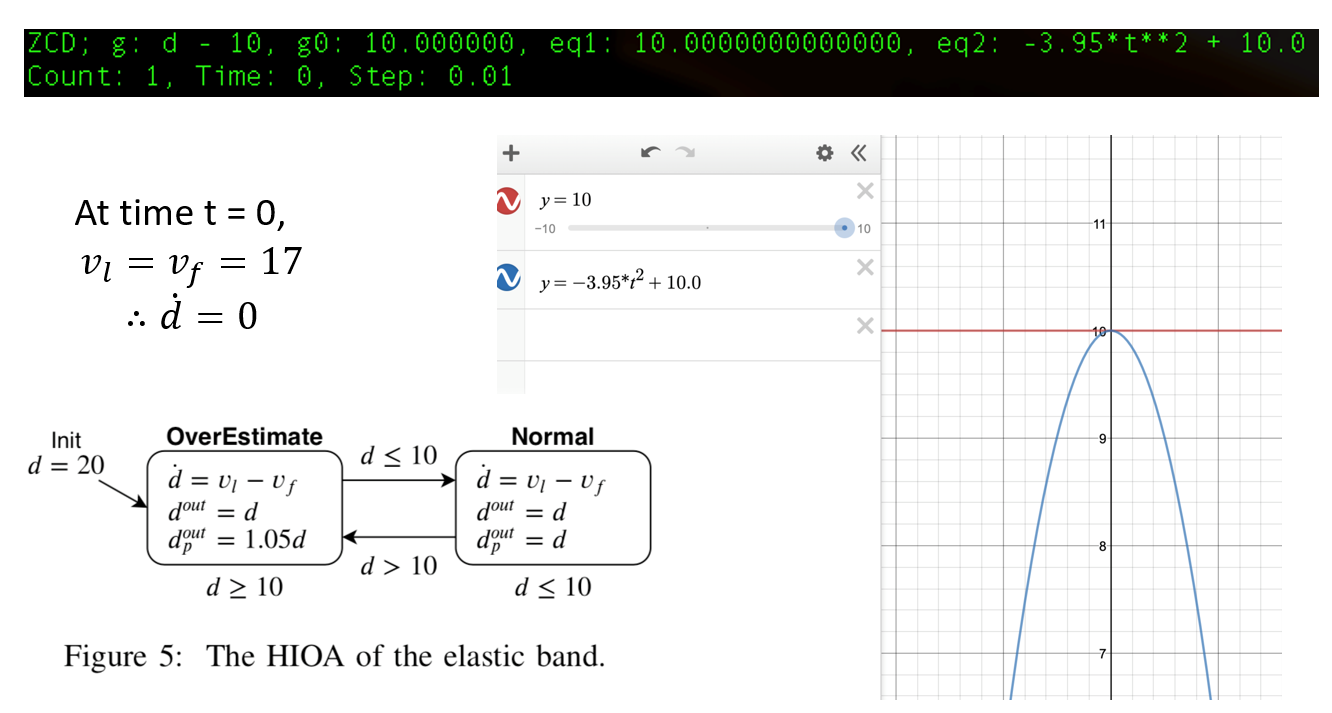
\includegraphics[width=1\textwidth]{./fig/inefficiency.png}
	\end{figure}
\end{frame}
